\documentclass{beamer}
\usetheme{Rochester}
\usecolortheme{dove}
\usefonttheme{serif}
\usepackage{multimedia}
\usepackage{modiagram}
\usepackage[version=4]{mhchem}
\usepackage{physics}
\usepackage{mathtools}
\usepackage{siunitx}
\usepackage{pifont}
\usepackage{adjustbox}
\usepackage{graphicx}
\usepackage{gensymb}
\usepackage{braket}

\definecolor{shiv_purple}{rgb}{0.6       ,  0.19607843,  0.8}
\definecolor{shiv_blue}{rgb}{0.11764706,  0.56470588,  1.}
\definecolor{shiv_green}{rgb}{0.        ,  0.57647059,  0.23529412}
\definecolor{shiv_yellow}{rgb}{0.97647059,  0.75686275,  0.1372549}
\definecolor{shiv_orange}{rgb}{1.        ,  0.54901961,  0.}
\definecolor{shiv_red}{rgb}{0.93333333,  0.20784314,  0.18039216}
\definecolor{shiv_gray}{rgb}{0.72156863,  0.71764706,  0.73333333}
%'darkorchid', 'dodgerblue', '00933C', 'FCCB09', 'darkorange', 'EE352E'

\setbeamercolor{itemize item}{fg=black}
\setbeamercolor{itemize subitem}{fg=black}
\setbeamercolor{itemize subsubitem}{fg=black}
\setbeamercolor{title}{fg=shiv_blue}
\setbeamercolor{frametitle}{fg=black}
\setbeamercolor{footline}{fg=black}

\makeatother
\setbeamertemplate{footline}
{%
  \leavevmode%
    \hspace{1em}\color{shiv_gray}{\insertshortauthor}\hfill{\insertsection}\hfill{\insertframenumber/\inserttotalframenumber}\hspace{1em}
    \vspace{1ex}
}
\makeatletter

\DeclareSIUnit{\cal}{cal}

\newcommand\blfootnote[1]{%
  \begingroup
  \renewcommand\thefootnote{}\footnote{#1}%
  \addtocounter{footnote}{-1}%
  \endgroup
}
\usepackage{booktabs}
\usepackage[style=chem-acs]{biblatex}

\usepackage{braket}
\usepackage{mathtools}
\DeclarePairedDelimiter\cbra{\lparen}{\rvert}
\DeclarePairedDelimiter\cket{\lvert}{\rparen}
\DeclarePairedDelimiterX\cinner[2]{\lparen}{\rparen}{#1 \delimsize\vert #2}
% \DeclarePairedDelimiterX\cbraket[2]{(}{)}{#1 \delimsize\vert #2}
\DeclarePairedDelimiterX\cbraket[3]{\lparen}{\rparen}%
{#1 \delimsize\vert #2 \delimsize\vert #3}

\addbibresource{references.bib}

\setbeamertemplate{enumerate items}[default]
\setbeamertemplate{itemize items}[circle]
\setbeamertemplate{navigation symbols}{}
\setbeamertemplate{frametitle}{\vspace{-1.25cm}\centering \LARGE{\insertframetitle}\\ \insertframesubtitle}
\setbeamerfont{footnote}{size=\tiny}

\usepackage{enumitem}
\setitemize{label=\usebeamerfont*{itemize item}%
  \usebeamercolor[fg]{itemize item}
  \usebeamertemplate{itemize item}}

\usepackage{microtype}

\title{{\Huge Density Functional Theory}}
\author[Shiv]{Shiv Upadhyay}
\institute{\normalsize{\textit{University of Pittsburgh}
\vspace{0.3cm}}}
\begin{document}
\frame{\vspace{-1.25cm}\titlepage}
%%%%%%%%%%%%%%%%%%%%%%%%%%%%%%%%%%%%%%%%%%%%%%%%%%%%%%
\begin{frame}[t]{Hartree-Fock reminder}
Molecular electronic Hamiltonian
\begin{equation*}
H = T + V_{ee} + V_{en}
\end{equation*}
\pause
Make the approximation that the electrons interact with the \emph{mean field} of the other electrons\\
\pause
\begin{equation*}
H = T + V_{ee} + V_{en}
\end{equation*}
\pause
\begin{align*}
F &= H^{\mathrm{core}} + G \\
G_{\lambda\sigma} &= \sum_{\lambda\sigma} P_{\lambda\sigma}[2(\mu\nu|\lambda\sigma) - (\mu\lambda|\nu\sigma)]
\end{align*}
\end{frame}
%%%%%%%%%%%%%%%%%%%%%%%%%%%%%%%%%%%%%%%%%%%%%%%%%%%%%%
\begin{frame}[t]{Why do we need DFT???}
HF neglects \emph{electron correlation}\\ \vfill
\pause
Electron correlation can be static (multiple near equal energy configurations) and dynamics electron/electron reactions. \\ \vfill
\begin{equation}
E_{\mathrm{corr}} = E_{\mathrm{HF}} - E_{\mathrm{TRUE}}
\end{equation}
\pause
\vfill
This happens because in reality the electrons don't interact with the mean field of the electrons; they interact with all the other electrons.
\vfill
\end{frame}
%%%%%%%%%%%%%%%%%%%%%%%%%%%%%%%%%%%%%%%%%%%%%%%%%%%%%%
\begin{frame}[t]{1998 Nobel Prize}
\begin{figure}
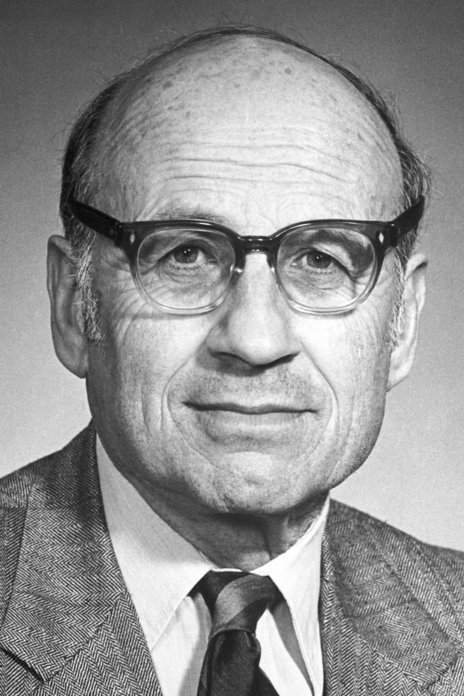
\includegraphics[width=0.5\textwidth,height=\textheight,keepaspectratio]{kohn.jpg}
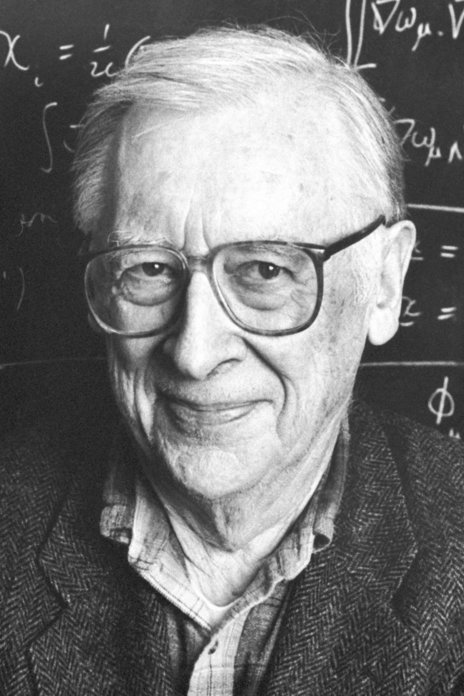
\includegraphics[width=0.5\textwidth,height=\textheight,keepaspectratio]{pople.jpg}
\end{figure}
\end{frame}
%%%%%%%%%%%%%%%%%%%%%%%%%%%%%%%%%%%%%%%%%%%%%%%%%%%%%%
\begin{frame}[t]{Density as a fundemental object}

\end{frame}
%%%%%%%%%%%%%%%%%%%%%%%%%%%%%%%%%%%%%%%%%%%%%%%%%%%%%%
\end{document}
